% Overall methodology of CONCLAVE.  Compile: pdflatex fig_method.tex
\documentclass[tikz,border=2pt]{standalone}
\usepackage{mathptmx}
\usepackage{amsmath,amssymb}
\usetikzlibrary{positioning,arrows.meta,calc,fit,backgrounds}
\definecolor{cData}{HTML}{DCEAF7}\definecolor{bData}{HTML}{2E6DA4}
\definecolor{cEng}{HTML}{DDF1EC}\definecolor{bEng}{HTML}{1E8A70}
\definecolor{cFeat}{HTML}{E9F3DA}\definecolor{bFeat}{HTML}{5E8C2A}
\definecolor{cTrain}{HTML}{FCEBD6}\definecolor{bTrain}{HTML}{C0661A}
\definecolor{cAgent}{HTML}{ECE4F5}\definecolor{bAgent}{HTML}{6A3FA0}
\definecolor{cEval}{HTML}{EEEEEE}\definecolor{bEval}{HTML}{555555}
\begin{document}
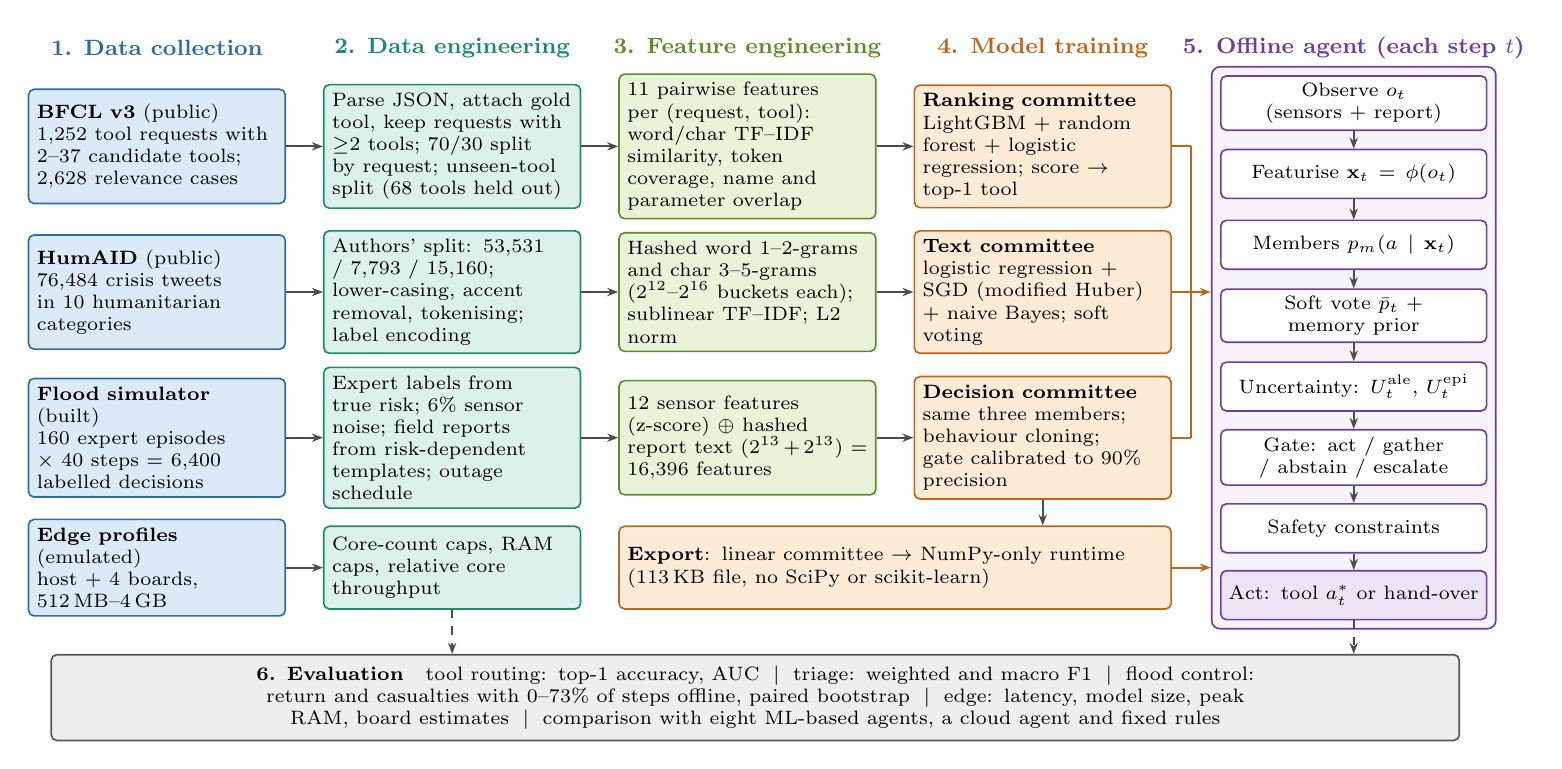
\begin{tikzpicture}[
  font=\scriptsize,
  box/.style={draw=#1, rounded corners=2pt, line width=0.6pt, align=left,
              text width=3.05cm, inner sep=3pt, minimum height=1.45cm,
              execute at begin node={\hyphenpenalty=10000\exhyphenpenalty=10000}},
  hdr/.style={font=\footnotesize\bfseries, text=#1, align=center},
  arr/.style={-{Stealth[length=4pt]}, line width=0.7pt, draw=black!70},
  stp/.style={draw=bAgent, fill=white, rounded corners=2pt, line width=0.6pt,
               text width=3.2cm, align=center, inner sep=2.5pt, minimum height=0.62cm,
               execute at begin node={\hyphenpenalty=10000\exhyphenpenalty=10000}},
]
% column x positions
\def\xa{0}\def\xb{3.75}\def\xc{7.5}\def\xd{11.25}\def\xe{15.2}
% ---------------- headers
\node[hdr=bData]  at (\xa,1.25) {1. Data collection};
\node[hdr=bEng]   at (\xb,1.25) {2. Data engineering};
\node[hdr=bFeat]  at (\xc,1.25) {3. Feature engineering};
\node[hdr=bTrain] at (\xd,1.25) {4. Model training};
\node[hdr=bAgent] at (\xe,1.25) {5. Offline agent (each step $t$)};
% ---------------- row 1: BFCL
\node[box=bData, fill=cData] (a1) at (\xa,0) {\textbf{BFCL v3} (public)\\ 1{,}252 tool requests with 2--37 candidate tools; 2{,}628 relevance cases};
\node[box=bEng, fill=cEng] (b1) at (\xb,0) {Parse JSON, attach gold tool, keep requests with $\geq$2 tools; 70/30 split by request; unseen-tool split (68 tools held out)};
\node[box=bFeat, fill=cFeat] (c1) at (\xc,0) {11 pairwise features per (request, tool): word/char TF--IDF similarity, token coverage, name and parameter overlap};
\node[box=bTrain, fill=cTrain] (d1) at (\xd,0) {\textbf{Ranking committee}\\ LightGBM + random forest + logistic regression; score $\to$ top-1 tool};
% ---------------- row 2: HumAID
\node[box=bData, fill=cData] (a2) at (\xa,-1.85) {\textbf{HumAID} (public)\\ 76{,}484 crisis tweets in 10 humanitarian categories};
\node[box=bEng, fill=cEng] (b2) at (\xb,-1.85) {Authors' split: 53{,}531 / 7{,}793 / 15{,}160; lower-casing, accent removal, tokenising; label encoding};
\node[box=bFeat, fill=cFeat] (c2) at (\xc,-1.85) {Hashed word 1--2-grams and char 3--5-grams ($2^{12}$--$2^{16}$ buckets each); sublinear TF--IDF; L2 norm};
\node[box=bTrain, fill=cTrain] (d2) at (\xd,-1.85) {\textbf{Text committee}\\ logistic regression + SGD (modified Huber) + naive Bayes; soft voting};
% ---------------- row 3: simulator
\node[box=bData, fill=cData] (a3) at (\xa,-3.7) {\textbf{Flood simulator} (built)\\ 160 expert episodes $\times$ 40 steps = 6{,}400 labelled decisions};
\node[box=bEng, fill=cEng] (b3) at (\xb,-3.7) {Expert labels from true risk; 6\% sensor noise; field reports from risk-dependent templates; outage schedule};
\node[box=bFeat, fill=cFeat] (c3) at (\xc,-3.7) {12 sensor features (z-score) $\oplus$ hashed report text ($2^{13}+2^{13}$) = 16{,}396 features};
\node[box=bTrain, fill=cTrain] (d3) at (\xd,-3.7) {\textbf{Decision committee}\\ same three members; behaviour cloning; gate calibrated to 90\% precision};
% ---------------- row 4: edge
\node[box=bData, fill=cData, minimum height=1.05cm] (a4) at (\xa,-5.35) {\textbf{Edge profiles} (emulated)\\ host + 4 boards, 512\,MB--4\,GB};
\node[box=bEng, fill=cEng, minimum height=1.05cm] (b4) at (\xb,-5.35) {Core-count caps, RAM caps, relative core throughput};
\node[box=bTrain, fill=cTrain, minimum height=1.05cm, text width=6.8cm] (d4) at ($(\xc,-5.35)!0.5!(\xd,-5.35)$) {\textbf{Export}: linear committee $\to$ NumPy-only runtime (113\,KB file, no SciPy or scikit-learn)};
% ---------------- arrows along rows
\foreach \r in {1,2,3}{
  \draw[arr] (a\r) -- (b\r); \draw[arr] (b\r) -- (c\r); \draw[arr] (c\r) -- (d\r);}
\draw[arr] (a4) -- (b4);
\draw[arr] (d3.south) -- (d3.south |- d4.north);
% ---------------- agent column
\node[stp] (s1) at (\xe,0.55)  {Observe $o_t$ (sensors + report)};
\node[stp] (s2) at (\xe,-0.35) {Featurise $\mathbf{x}_t=\phi(o_t)$};
\node[stp] (s3) at (\xe,-1.25) {Members $p_m(a\mid\mathbf{x}_t)$};
\node[stp] (s4) at (\xe,-2.15) {Soft vote $\bar p_t$ + memory prior};
\node[stp] (s5) at (\xe,-3.05) {Uncertainty: $U^{\mathrm{ale}}_t$, $U^{\mathrm{epi}}_t$};
\node[stp] (s6) at (\xe,-3.95) {Gate: act / gather / abstain / escalate};
\node[stp] (s7) at (\xe,-4.85) {Safety constraints};
\node[stp, fill=cAgent] (s8) at (\xe,-5.7) {Act: tool $a^\ast_t$ or hand-over};
\foreach \i/\j in {s1/s2,s2/s3,s3/s4,s4/s5,s5/s6,s6/s7,s7/s8}{\draw[arr] (\i) -- (\j);}
\begin{scope}[on background layer]
\node[fill=cAgent!45, draw=bAgent, rounded corners=3pt, line width=0.6pt,
      fit=(s1)(s8), inner sep=3pt] (agentbox) {};
\end{scope}
% committees feed the agent
\coordinate (feed) at ($(agentbox.west)+(-0.25,0)$);
\foreach \r in {1,2,3}{\draw[line width=0.7pt, draw=bTrain] (d\r.east) -- (d\r.east -| feed);}
\draw[line width=0.7pt, draw=bTrain] (d1.east -| feed) -- (d3.east -| feed);
\draw[arr, draw=bTrain] (d2.east -| feed) -- (agentbox.west |- d2.east);
\draw[arr, draw=bTrain] (d4.east) -- (agentbox.west |- d4.east);
% ---------------- evaluation band
\node[draw=bEval, fill=cEval, rounded corners=2pt, line width=0.6pt, text width=17.6cm,
      align=center, inner sep=4pt, execute at begin node={\hyphenpenalty=10000}] (ev) at (7.6,-7.0)
{\textbf{6. Evaluation}\quad tool routing: top-1 accuracy, AUC \;$\mid$\; triage: weighted and macro F1
 \;$\mid$\; flood control: return and casualties with 0--73\% of steps offline, paired bootstrap
 \;$\mid$\; edge: latency, model size, peak RAM, board estimates
 \;$\mid$\; comparison with eight ML-based agents, a cloud agent and fixed rules};
\draw[arr, dashed] (b4.south) -- (b4.south |- ev.north);
\draw[arr, dashed] (s8.south) -- (s8.south |- ev.north);
\end{tikzpicture}
\end{document}
